\documentclass[10pt,a4paper]{article}

\usepackage[utf8]{inputenc}
\usepackage[english]{babel}
\usepackage{amsmath}
\usepackage{amsfonts}
\usepackage{amssymb}
\usepackage{graphicx}


% меняем поля
\usepackage{geometry}
\geometry{left=3cm}
\geometry{right=2cm}
\geometry{top=2cm}
\geometry{bottom=2cm}

\begin{document}

\begin{center} 

\large SAINT-PETERSBURG STATE POLYTECHNICAL UNIVERSITY

\large Department of Computer Systems and Software engineering \\[8.5cm] 

\huge ESSAY \\[0.6cm] % название работы, затем отступ 0,6см
\large for second lecture\\
\large Discipline: "Information security"\\[4.5cm]

\end{center} 

\begin{flushright}
Performed: student gr. 53501/2 \\
Ponomarev M.A \\[1.0cm]


Teacher \\
Vilegzanina K.D
\end{flushright}


\vfill 

\begin{center} 
\large Saint-Petersburg \\
2015
\end{center} 

\thispagestyle{empty}

\newpage


\begin{center}


\begin{Large}
\textbf{Essay cover three themes:}

\begin{itemize}
	\item Improving Efficiency of Spam Detection using Economic Model
	\item Enterprise Risk Assessment Based on Compliance Reports and \\ 						  Vulnerability Scoring Systems
	 \item Protecting Enterprise Networks through Attack Surface Expansion
\end{itemize} 
\end{Large}
\end{center}
\bigskip

\section{First theme}

The first theme ensures us about significant impact of email spam on our life. As well as that, it states that econimic lifts and declines lead to increasing or, opposite, decreasing threats of email spamming. One of way to detect email spamming is to include a novel economic metric, based on the underlying spam economic system, to assist detectors in keeping their false positives at bay by associating detection accuracy to the spammer’s cost.  

\begin{figure}[hhh!]
	\begin{center}
		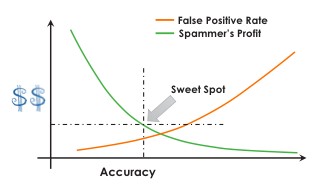
\includegraphics[width=10cm]{img/eco_metric}
	\end{center}
	\vspace{-5mm}\caption{Economic metric}
\end{figure}

Main idia is that spammer program spend some money to achieve some desired utility. Constraining the economic model using the detection features provides a relationship between detection accuracy and spammer’s cost. So that spam detectors suffer from the inherent tradeoff between accuracy and efficiency. Since, spam is all about earning money, to deal with it:
\begin{itemize}
	\item \textbf{Created} an economic metric by associating the detection accuracy of the detectors with the spammer’s cost.
	\item \textbf{Developed} a mechanism to identify effective spam detection features (like IDT) using K directed divergence analysis, followed by the use of ROC curves to evaluate the performance of IDT based detector
	\item \textbf{Developed} a spam economic model that calculates the spammer utility in terms of the number of spam emails sent by the spammer. Fur- ther constraining this utility with the IDT feature, we have added a cost sense into the detector to focus on increasing spammer’s cost rather than just the detection accuracy.
\end{itemize}

\newpage


\section{Second theme}

The second theme is about risk assessment. Risk assessment aims to provide consistent recommendations to maximize the protection of organization assets. There are two main documents to provide standarts of risk management:
\begin{itemize}
	\item \textbf{The Security Content Automation Protocol (SCAP)} provides standard specifications to communicate security information. 
	\item \textbf{The Extensible Configuration Checklist Description Format (XCCDF)} specifies a language to describe security checklists and collect com- pliance results of targeted systems.
\end{itemize}

Risk models define the risk factors to be assessed and the relationships among them. Typical risk factors include threat, vulnerability, impact, likelihood of exploit, and predisposing condition. Risk model defines the risk in terms of: 
 
\begin{itemize}
	\item The exploitability and impact scores reported by the vulnerability scoring systems.
	\item Hosts’ exposure that takes into con- sideration the network configuration and the vulnerabilities distribution. 
	\item The assets distribution in the network. 
\end{itemize} 
 
To calculate risk is used the total impact subscore and the integrity impact base score as in the case of Infidelity. The Risk of a particular host h formally is:

\begin{equation}
Risk(h) = A(h) * B(h) * \sum_v (\frac{\$[v, E]}{10} * \$[v, I])
\end{equation}
 
where $A(h)$ is the asset value of the host $h$.

\bigskip

This work investigates the feasibility of using security compliance reports along with universal vulnerability scores and network configuration in assessing the risk of cyberattacks.
 

\section{Third theme}

The third theme declares that it is critical to protect the enterprise assets from being stolen or compromised by internal and external attackers. Attack surface is a valuable metric that help administrators of enterprise networks to evaluate the risk and security of the entire network. 

Current theme is about research efforts usually focus on reducing the attack surface observed by the attackers. Attacks are devided by:
\begin{itemize}
	\item \textbf{Internal attack surface (IAS)} - the attack surface observed by the defenders
	\item \textbf{External attack surface (EAS)} - the attack that can be observed by the external unauthenticated attackers
\end{itemize}

A system’s attack surface is the set of ways in which an adversary can enter the system and potentially cause damage. There are three main ways of
expanding Attack Surface:
\begin{itemize}
	\item using Virtual Identities
	\item using Dynamic Virtual Networks
	\item using Secret Moving Proxy
\end{itemize}



\end{document}